\documentclass[14pt]{beamer}

\title[A Tour of Go]{\huge Let's Go!}
\author{Mansi Sharma}
\usetheme{Madrid}

\definecolor{deepblue}{HTML}{302B70}

\begin{document}

{
\begin{frame}
    \titlepage
    
\includegraphics[width=\linewidth]{img/golang.png}
\end{frame}
}

{
\begin{frame}
    \frametitle {What is Go?}
    \begin{center}
    \textcolor{deepblue}{Go is a \textcolor{red}{compiled}, \textcolor{green}{concurrent}, \textcolor{yellow}{garbage-collected}, \textcolor{blue}{statically typed} language developed at}
    \linebreak
    
\includegraphics[width=0.3\linewidth]{img/google.png}
    \end{center}
\end{frame}
}

{
\begin{frame}
    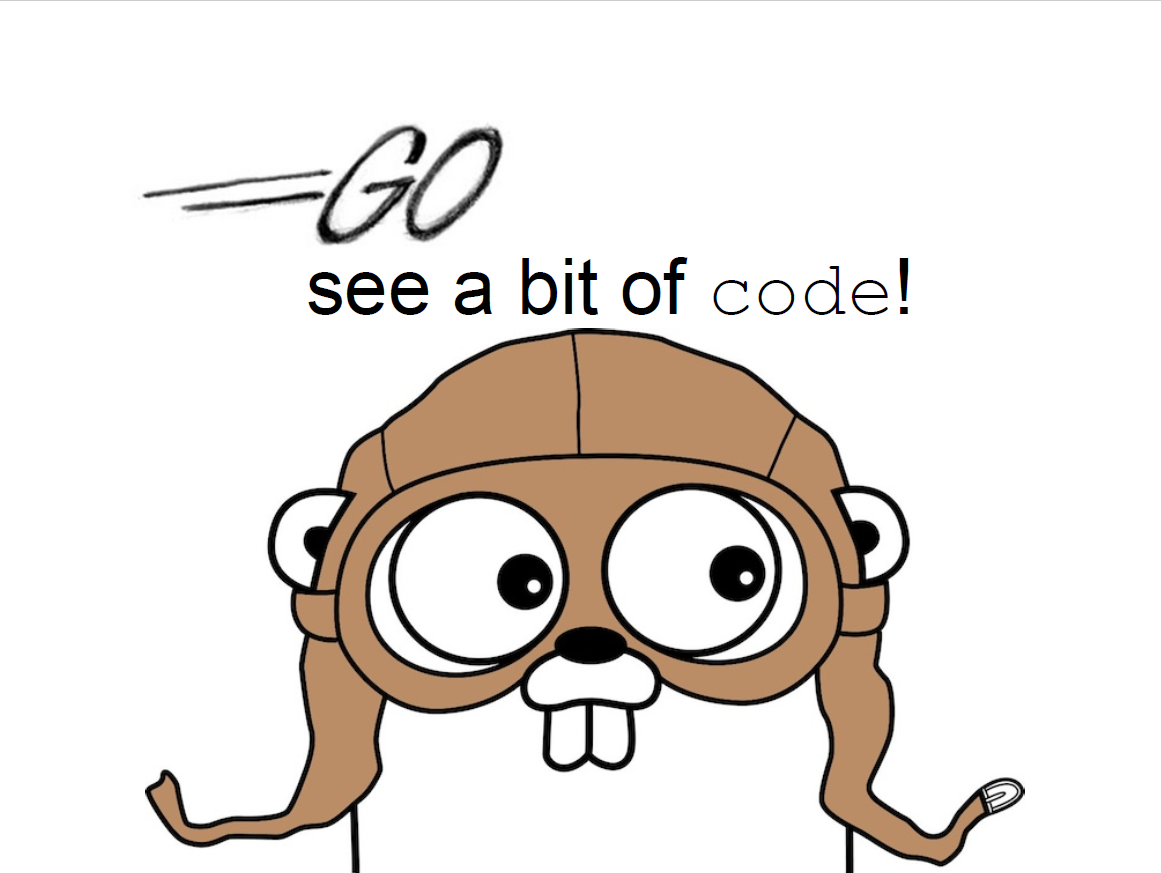
\includegraphics[width=\linewidth]{img/golang.PNG}
\end{frame}
}

{
\begin{frame}
    \frametitle{Hello, World!}
    \begin{itemize}
\item Programs start running in package main.
\item It is good style to use the factored import statement.
\item A name is exported if it begins with a capital letter.
    \end{itemize}
    \begin{center}
    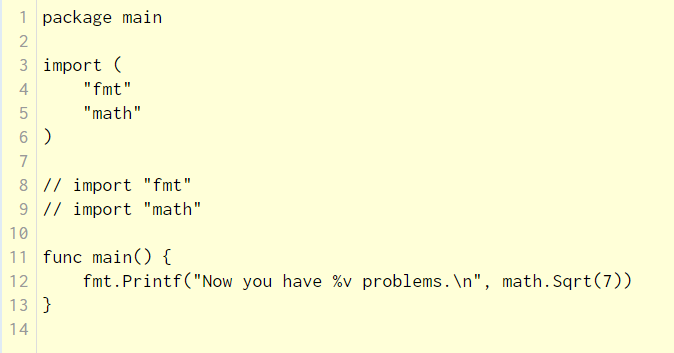
\includegraphics[width=0.7\linewidth]{img/introtogo.PNG}
    \end{center}
\end{frame}
}

{
\begin{frame}
    \frametitle{Variables}
    \begin{itemize}
\item The var instruction declares a list of variables
\item The type is informed at the end
\item The var instruction could includes initializers, 1 per variable. In this case, the type could be ommited
    \end{itemize}
    \begin{center}
    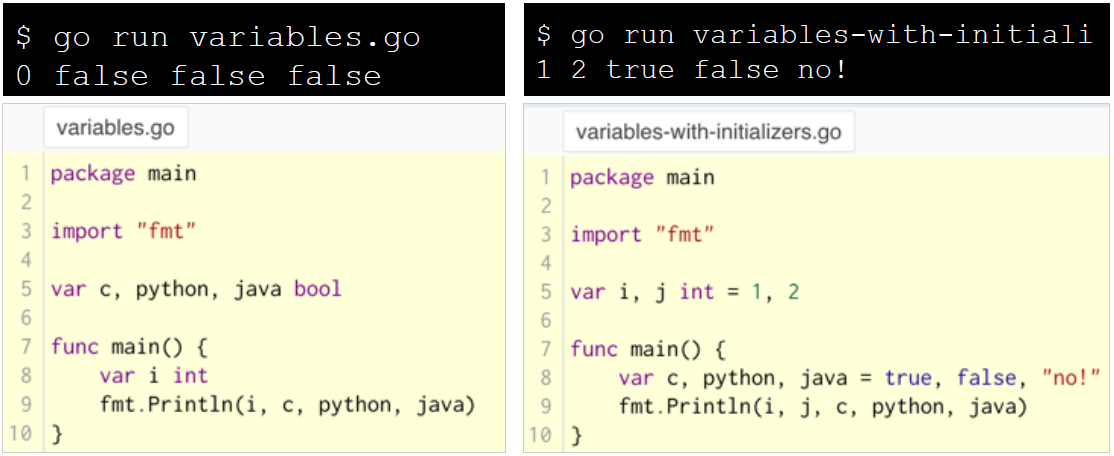
\includegraphics[width=\linewidth]{img/variables.PNG}
    \end{center}
\end{frame}
}

{
\begin{frame}
    \frametitle{Short Variable Declarations}
    \begin{itemize}
\item Inside a function, the short attribution instruction := can be used instead of a var declaration
    \end{itemize}
    \begin{center}
        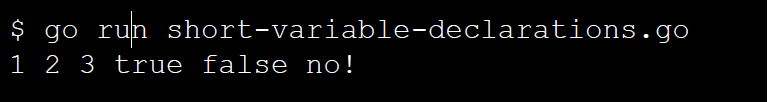
\includegraphics[width=0.6\linewidth]{img/shortdeclarationcommand.PNG}
        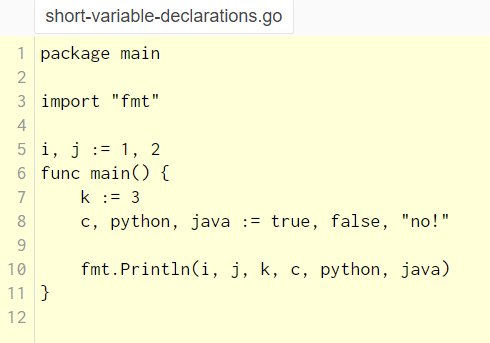
\includegraphics[width=0.6\linewidth]{img/shortdeclaration.PNG}
    \end{center}
\end{frame}
}

{
\begin{frame}
    \frametitle{Constants}
    \begin{itemize}
\item Constants are declared like variables but with keyword const
\item Can not use the syntx :=
    \end{itemize}
    \begin{center}
    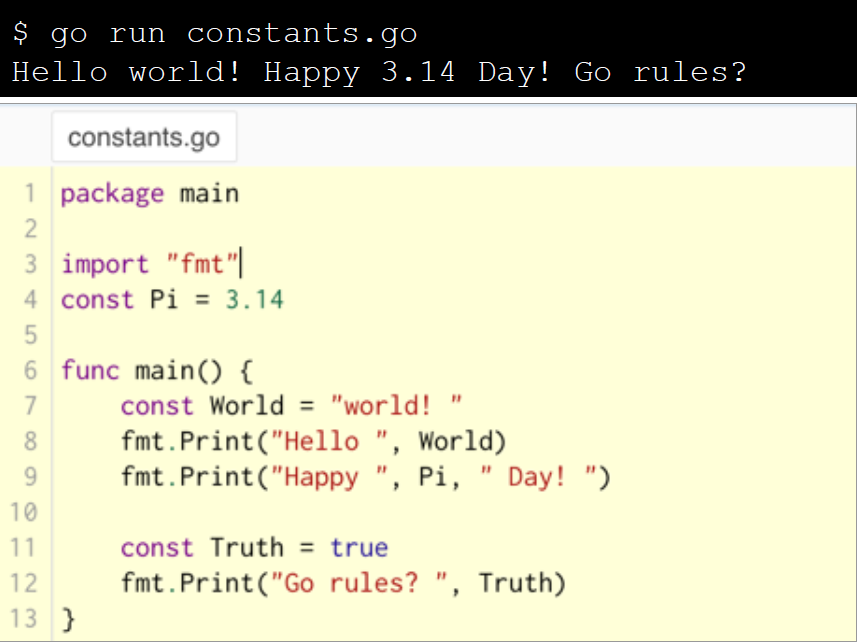
\includegraphics[width=0.6\linewidth]{img/constants.PNG}
    \end{center}
\end{frame}
}

{
\begin{frame}
    \frametitle{Functions}
    \begin{itemize}
\item Type comes after the parameter name, like variables
\item Shorten (x int, y int) to (x, y int)
    \end{itemize}
        \begin{columns}
            \begin{column}{0.5\textwidth}
                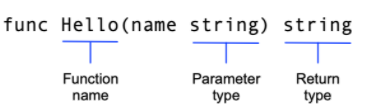
\includegraphics[width=\linewidth]{img/function.PNG}
                \linebreak
                \linebreak
                \linebreak
                \linebreak
                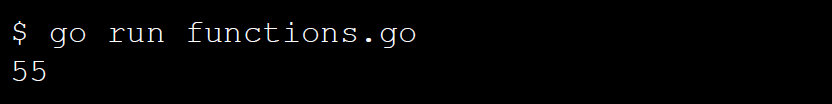
\includegraphics[width=\linewidth]{img/functionscommand.PNG}
            \end{column}
            \begin{column}{0.5\textwidth}
                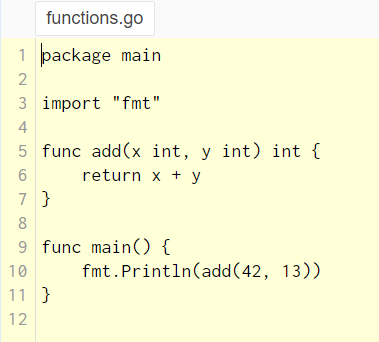
\includegraphics[width=\linewidth]{img/functions.PNG}
            \end{column}
        \end{columns}
\end{frame}
}

{
\begin{frame}
    \frametitle{Multiple Return Values}
    \begin{itemize}
        \item A function can have multiple return values
    \end{itemize}
    \begin{center}
        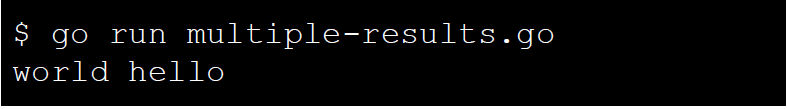
\includegraphics[width=0.65\linewidth]{img/multipleresultscommand.PNG}
        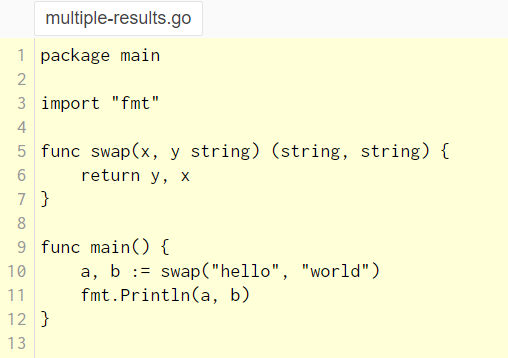
\includegraphics[width=0.65\linewidth]{img/multipleresults.PNG}
    \end{center}
\end{frame}
}

{
\begin{frame}
    \frametitle{Looping For}
    \begin{itemize}
        \item Go has only one looping construct, the for loop
        \item No parentheses required, braces are always required
        \item The init and post statements are optional
    \end{itemize}
    \begin{center}
        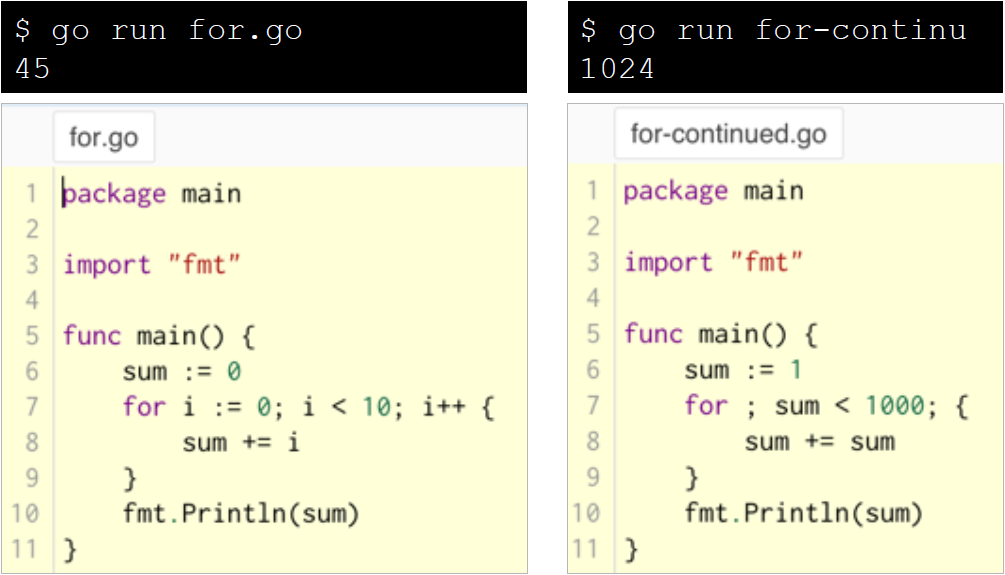
\includegraphics[width=0.8\linewidth]{img/for.PNG}
    \end{center}
\end{frame}
}

{
\begin{frame}
    \frametitle{For is Go's "while" and forever}
    \begin{itemize}
        \item Semicolon can be removed and you will have while
        \item for can run forever
    \end{itemize}
    \begin{center}
        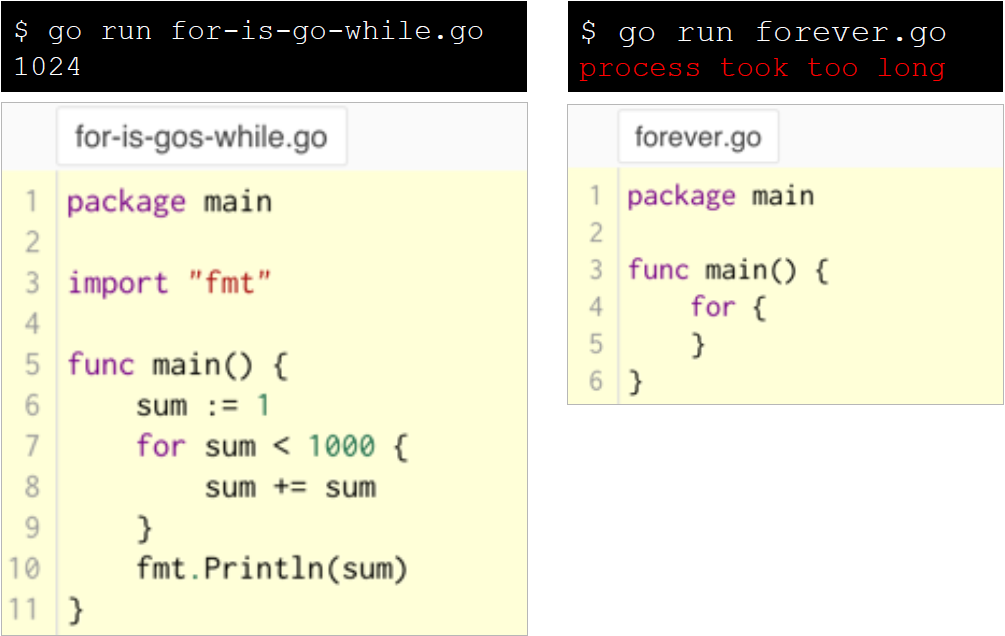
\includegraphics[width=0.8\linewidth]{img/while.PNG}
    \end{center}
\end{frame}
}

{
\begin{frame}
    \frametitle{if Condition}
    \begin{itemize}
        \item No parentheses required, braces are always required
    \end{itemize}
    \begin{columns}
        \begin{column}{0.5\textwidth}
        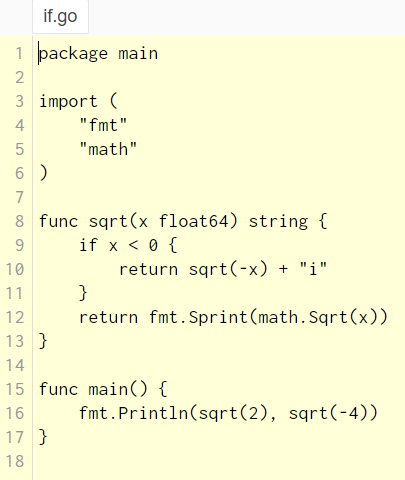
\includegraphics[width=\linewidth]{img/if.PNG}
        \end{column}
        \begin{column}{0.5\textwidth}
        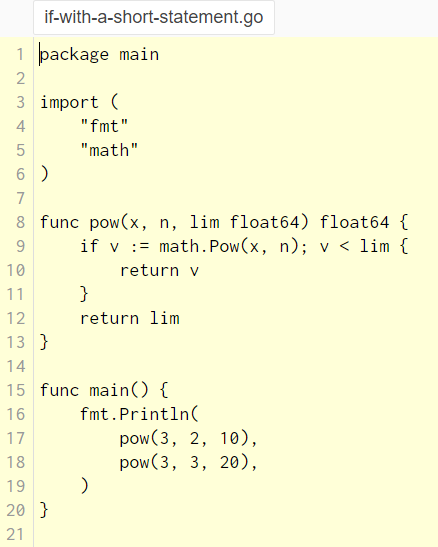
\includegraphics[width=0.9\linewidth]{img/ifshort.PNG}
        \end{column}
    \end{columns}
\end{frame}
}

{
\begin{frame}
    \frametitle{Switch}
    \begin{itemize}
        \item only runs the selected case, not all the cases that follow
        \item break statement is not required
    \end{itemize}
    \begin{columns}
        \begin{column}{0.5\textwidth}
        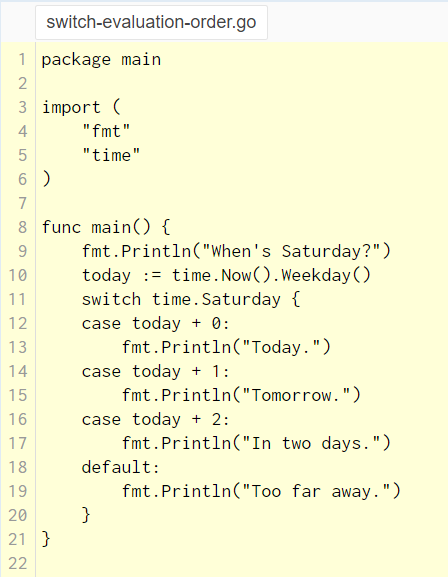
\includegraphics[width=0.75\linewidth]{img/switch1.PNG}
        \end{column}
        \begin{column}{0.5\textwidth}
        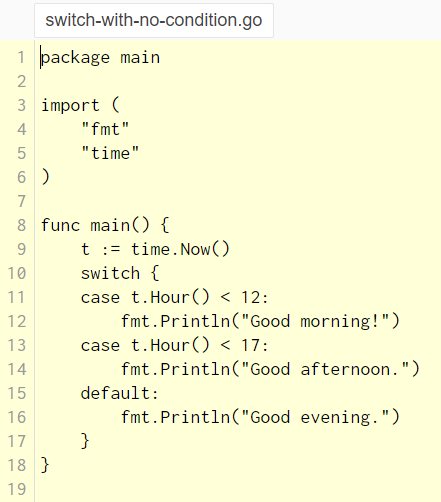
\includegraphics[width=0.8\linewidth]{img/switch2.PNG}
        \end{column}
    \end{columns}
\end{frame}
}

{
\begin{frame}
    \frametitle{Defer}
    \begin{itemize}
        \item Semicolon can be removed and you will have while
        \item for can run forever
    \end{itemize}
    \begin{center}
        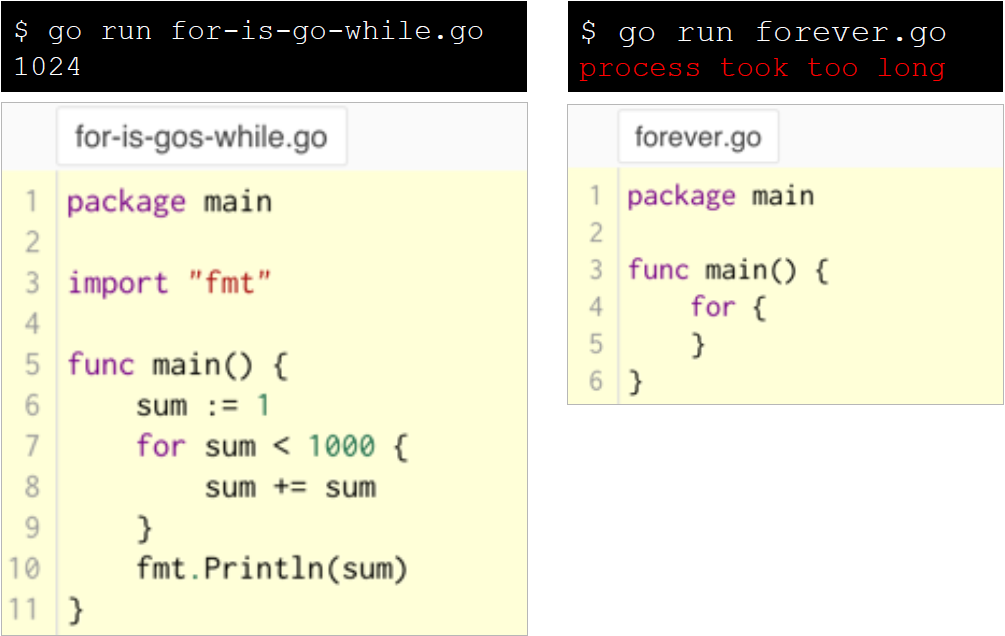
\includegraphics[width=0.8\linewidth]{img/while.PNG}
    \end{center}
\end{frame}
}

{
\begin{frame}
    \frametitle{Stacking Defer}
    \begin{itemize}
        \item Deferred function calls are pushed onto a stack
    \end{itemize}
    \begin{columns}
        \begin{column}{0.5\textwidth}
        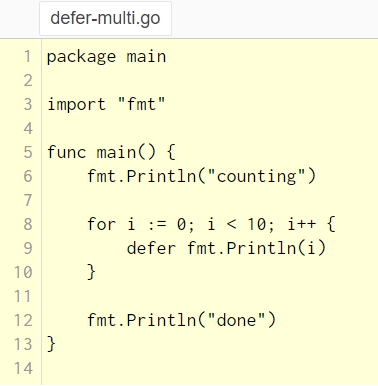
\includegraphics[width=0.9\linewidth]{img/stackdefer.PNG}
        \end{column}
        \begin{column}{0.5\textwidth}
        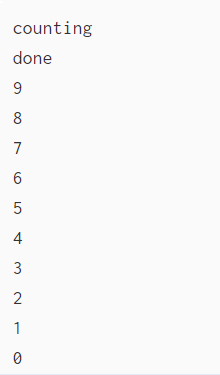
\includegraphics[width=0.5\linewidth]{img/defeeoutput.PNG}
        \end{column}
    \end{columns}
\end{frame}
}

{
\begin{frame}
        
\includegraphics[width=\textwidth]{img/questions.PNG}
\end{frame}
}

\end{document}
